\chapter{Présentation du projet}

	\section{Présentation général de l'application}
        Magic Book est un éditeur de livre permettant de créer un livre à choix multiples pouvant contenir des conditions pour certains d'entre eux, des choix aléatoires, des combats, etc.\\
        L'utilisateur peut donc créer des paragraphes, appelés des "noeuds", reliés entre eux par des liens. Ces liens peuvent être bloqué par des prérequis, permettant ainsi que l'utilisateur rajoute de la difficulté dans l'histoire. L'ajout de personnages, d'items et de compétences sont aussi disponible, répondant au mieux à l'imagination de l'utilisateur.
        Une fois le livre créé, l'utilisateur peut alors obtenir une estimation de la difficulté du livre en choisissant l'option correspondante dans la barre de menu en haut. Cette difficulté est ensuite affichée dans le panel des stats. Une option "Jouer" est également disponible, permettant ainsi de jouer à l'histoire créée. Enfin, il est également possible d'exporter le livre dans un format texte.\\
        Bien entendu, il est possible d'enregistrer le livre afin de le réouvrir pour continuer l'édition de celui-ci.\\

	\section{Présentation de l'application}

		\begin{center}
			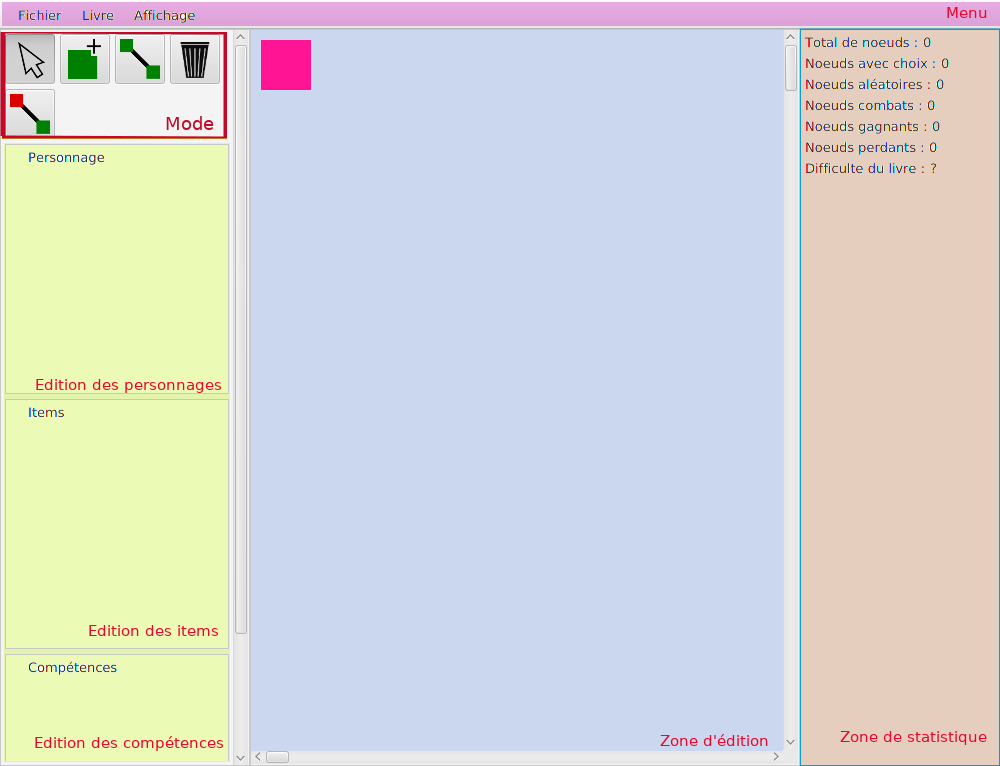
\includegraphics[width=10cm]{img/magicBook.png}
		\end{center}

		L'application comprend quatre parties. Elle est tout d'abord constituer d'un menu, permettant ainsi d'utiliser toutes les options de cette application, que cela soit sur son enregistrement, comme à son afichage ou encore, à sa jouabilité.
		Elle contient ensuite des boutons permettant à l'utilisatuer de changer de mode. En dessous de ces boutons, des tableaux sont affichés. Ces tableaux sont scrollable et contiennent des personnages, items, compétences à ajouter dans le livre.
		Il y a ensuite la zone d'édition. Cette zone contient tout ce qui vas être afficher dans le livre : prélude, paragraphe, personnages, items...
		La zone à droite permet à l'utilisateur d'avoir une vue global sur le livre: nombre de noeud totaux, nombre de noeuds en fonction de son type, difficulté du livre...
